%!TEX ROOT=../ctutest.tex

\chapter{Current Contribution}
\label{chap:contribution}

\textit{We have collected novel data, emulated and scraped inavailable datasets making them public or readying them for doing so, we have established numerous sota models and are currently working on establishing the topic of claim generation as a summarization-related NLP task.
We are also readying metrics for fact-checking, experimenting with them and so on and soforth.}

\section{Datasets}
\label{sec:pretrain}
\subsection{CsFEVER}
\subsection{CTKFacts}
\subsection{Other NLP datasets in West Slavic languages}
\begin{enumerate}
    \item {\techbf Translated NLI datasets} -- SNLI, ANLI, MultiNLI, 
    \item SmeSum, CTKSum, CsFEVERSum
    \item Polish summarization data
\end{enumerate}
\section{Models}
\label{sec:models}
\section{Publications}
\label{sec:models}
\section{Applications}
\label{sec:models}

\begin{figure}
    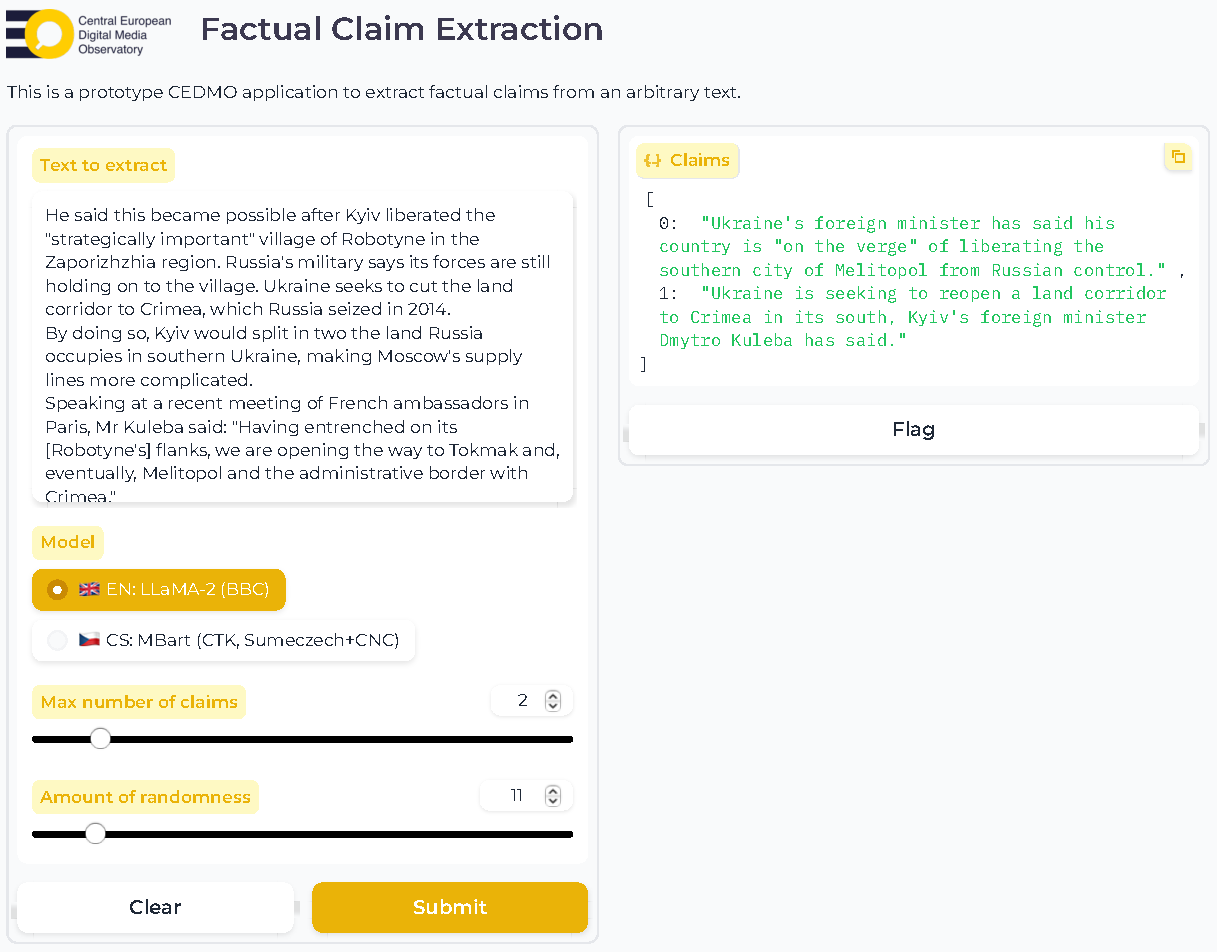
\includegraphics[width=16cm]{fig/cedmo.pdf}
    \caption{Factual claim extraction application done for the CEDMO project}
    \label{fig:framework}
\end{figure}

Here we will show off the demonstration tools, as well as our open-source platform \url{https://fcheck.fel.cvut.cz} and currently running claim extraction tools. 